% Copyright 2021 Adina-Maria Amzarescu

\documentclass[12pt,twoside]{article} 

\usepackage{tikz}
\usepackage{textcomp}
\usepackage[siunitx]{circuitikz}
\usepackage{siunitx}
\usepackage{systeme}
\usepackage{graphicx}
\usepackage{listings}
\usepackage{float}
\renewcommand{\contentsname}{Table of contents}


\begin{document}

\title{\begin{huge}
Electrical Circuit Project
\end{huge}\\
{\small -- Fundamentals of Electrical Engineering -- }}
\author{{\em Adina-Maria Amzărescu} \\ \\
311CA, 
Faculty of Automatic Control and Computer Science\\
University POLITEHNICA of Bucharest \\ \\
adina.amzarescu@stud.acs.upb.ro\\}
\date{May 2021} 
\maketitle

\newpage

\tableofcontents
\newpage

\section{The circuit}

The circuit:
\begin{center}
\begin{circuitikz}[european]
\draw (0, 2) to[R, l_=$R_3$,a^=8<\ohm>] (0, 4);
\draw[red] (2.5, 4) to[R, l_=$R_1$,a^=10<\ohm>, color=red] (6.5, 4);
\draw[red] (6.5, 4) to[R, l_=$R_4$,a^=6<\ohm>, color=red] (6.5, 0);
\draw[red] (2.5, 4) to[R, l_=$R_2$,a^=8<\ohm>, color=red] (2.5, 2.5);
\draw (2.5, 0) to[R, l_=$R_5$,a^=12<\ohm>] (4.5, 0);
\draw[red] (2.5, 2.5) to[V<=15V, color=red] (2.5, 0);
\draw (6.5,6.5) to[V<=30V] (2.5,6.5);
\draw (0,2) to[V<=15V] (0,0);
\draw (2.5,6.5) to[short] (2.5,4)node[label={[yshift=0.2cm, xshift=-7]right:$(1)$}]{};
\draw (6.5, 6.5) to[short] (6.5,4)node[label={[yshift=0.2cm, xshift=-7]right:$(2)$}]{};
\draw (0,0) to[short] (2.5,0)node[label={[font=\footnotesize]below:$(4)$}] {};
\draw (0,4) to[short] (2.5,4);
\draw (6.5, 4) to[short] (9,4);
\draw (9, 0) to[short] (6.5,0)node[label={[font=\footnotesize]below:$(3)$}] {};
\draw (9, 4) to[I>=4A] (9, 0) node[label={[font=\footnotesize]}]{};
\draw (6.5, 0) to [I>=10A] (4.5,0) node[label={[font=\footnotesize]}]{};
\end{circuitikz}
\end{center}


Electric current intensity graph:
\begin{center}
\begin{circuitikz}
\draw (0, 0) to[short, i>=5A] (0, 4);
\draw (2.5, 4) to[short, i<=3A]  (6.5, 4);
\draw (6.5, 4) to[short, i>=6A](6.5, 0);
\draw (2.5, 4) to[short, i<=5A] (2.5, 0);
\draw (6.5,6.5) to[short] (2.5,6.5);
\draw (2.5,6.5) to[short] (2.5,4)node[label={[yshift=0.2cm, xshift=-7]right:$(1)$}]{};
\draw (6.5, 6.5) to[short, i>=13A] (6.5,4)node[label={[yshift=0.2cm, xshift=-7]right:$(2)$}]{};
\draw (0,0) to[short] (2.5,0)node[label={[font=\footnotesize]below:$(4)$}] {};
\draw (0,4) to[short] (2.5,4);
\draw (6.5, 4) to[short] (9,4);
\draw (9, 0) to[short] (6.5,0)node[label={[font=\footnotesize]below:$(3)$}] {};
\draw (9, 4) to[short, i>=4A] (9, 0) ;
\draw (6.5, 0) to[short, i>=10A] (2.5,0);
\end{circuitikz}
\end{center}


\newpage
Voltage graph:
\begin{center}
\begin{circuitikz}
\draw (0, 0) to[short, i>=25] (0, 4);
\draw (2.5, 4) to[short, i<=30]  (6.5, 4);
\draw (6.5, 4) to[short, i>=36](6.5, 0);
\draw (2.5, 4) to[short, i<=25] (2.5, 0);
\draw (6.5,6.5) to[short] (2.5,6.5);
\draw (2.5,6.5) to[short] (2.5,4)node[label={[yshift=0.2cm, xshift=-7]right:$(1)$}]{};
\draw (6.5, 6.5) to[short, i<=30] (6.5,4)node[label={[yshift=0.2cm, xshift=-7]right:$(2)$}]{};
\draw (0,0) to[short] (2.5,0)node[label={[font=\footnotesize]below:$(4)$}] {};
\draw (0,4) to[short] (2.5,4);
\draw (6.5, 4) to[short] (9,4);
\draw (9, 0) to[short] (6.5,0)node[label={[font=\footnotesize]below:$(3)$}] {};
\draw (9, 4) to[short, i>=36] (9, 0) ;
\draw (6.5, 0) to[short, i<=31] (2.5,0);
\end{circuitikz}
\end{center}




\section{Efficient Systematic Methods}
\begin{center}
\begin{tabular}{|m{10cm}|m{5cm}|}
\hline
Method & Number of equations\\
\hline\hline
Kirchhoff classic & $2L = 14$\\
\hline
Kirchhoff's current law & $L - N + 1 = 4$\\
\hline
Kirchhoff's voltage law & $N - 1 = 3$\\
\hline
String current & $L - N + 1 - n_{SIC} = 3$\\
\hline
Tensions in branches & $N - 1 - n_{SIT} = 2$\\
\hline
\end{tabular}
\end{center}
In the above circuit, there are 4 nodes, marked with numbers 
from 1 to 4 and 7 sides. At the same time, in the circuit 
there are an ideal current source (SIC) and an ideal voltage source (SIT).\\\\
The tree has N-1 = 3 branches, colored above with red, and N-1-$n_{SIT}$ = 2 sections.\\
The sections:\\
\(1.\) The first section is composed of: (1)$\rightarrow$(4) and (4)$\rightarrow$(3); branch:(4)$\rightarrow$(1).\\
\(2.\) The second section is composed of:(3)$\rightarrow$(4) and (3)$\rightarrow$(2); branch:(3)$\rightarrow$(2).
\newpage
Using the branch tension method. 
(the most efficient) It is efficient because 
it's necessarily to write only 2 Kirchhoff 
equations. 
If the string current method is use, there will be 3 equations. 
For the 2 chosen sections, the Kirchhoff's current law (1st law) is used, and more precisely in the (3) and (4) nodes.

\begin{equation}
\systeme*{
{1}:\frac{U_{41}+15}{8}+\frac{U_{41}+15}{8}=10,
{2}:\frac{U{32}}{6}+10=4}
\end{equation}
By calculating: $U_{41}=25V$ and $U_{32}=26V$ as can be seen in the voltage graph, written at the beginning.
\newpage
\section{Equivalent Voltage/Current Generator}
The initial circuit:
\begin{center}
\begin{circuitikz}[european]
\draw (0, 2) to[R, l_=$R_3$,a^=8<\ohm>] (0, 4);
\draw[red] (2.5, 4) to[R, l_=$R_1$,a^=10<\ohm>, color=red] (6.5, 4);
\draw[red] (6.5, 4) to[R, l_=$R_4$,a^=6<\ohm>, color=red] (6.5, 0);
\draw[red] (2.5, 4) to[R, l_=$R_2$,a^=8<\ohm>, color=red] (2.5, 2.5);
\draw (2.5, 0) to[R, l_=$R_5$,a^=12<\ohm>] (4.5, 0);
\draw[red] (2.5, 2.5) to[V<=15V, color=red] (2.5, 0);
\draw (6.5,6.5) to[V<=30V] (2.5,6.5);
\draw (0,2) to[V<=15V] (0,0);
\draw (2.5,6.5) to[short] (2.5,4)node[label={[yshift=0.2cm, xshift=-7]right:$(1)$}]{};
\draw (6.5, 6.5) to[short] (6.5,4)node[label={[yshift=0.2cm, xshift=-7]right:$(2)$}]{};
\draw (0,0) to[short] (2.5,0)node[label={[font=\footnotesize]below:$(4)$}] {};
\draw (0,4) to[short] (2.5,4);
\draw (6.5, 4) to[short] (9,4);
\draw (9, 0) to[short] (6.5,0)node[label={[font=\footnotesize]below:$(3)$}] {};
\draw (9, 4) to[I>=4A] (9, 0) node[label={[font=\footnotesize]}]{};
\draw (6.5, 0) to [I>=10A] (4.5,0) node[label={[font=\footnotesize]}]{};
\end{circuitikz}
\end{center}


\subsection{Equivalent Generator's Characteristic}

The idea is to find out the dependence of intensity, voltage 
and power in the R5 resistor. To do this, we make $ E_{equivalent}$ 
on the left loop, and $ R_{equivalent}$.
On the top loop, there is a SIT in 
parallel with a resistor, which results in the initial SIT, and on the right 
loop there is a SRC, which is turned into SRT. In the figure there is 
the data (after performing these operations).

\begin{center}
\begin{circuitikz}[european]
\draw(2.5, 4) to[V<=30V] (6.5, 4);
\draw (6.5, 4) to[R, l_=$R_4$,a^=6<\ohm>] (6.5, 2);
\draw(2.5, 4) to[R, l_=$R_2$,a^=4<\ohm>] (2.5, 2.5);
\draw (2.5, 0) to[R, l_=$R_5$,a^=12<\ohm>] (4.5, 0);
\draw (6.5, 0) to[V<=24V] (6.5, 2);
\draw (2.5, 2.5) to[V<=15V] (2.5, 0);
\draw (6.5, 0) to [I>=10A] (4.5,0) node[label={[font=\footnotesize]}]{};
\end{circuitikz}
\end{center}

Now it's time to calculate $ E_{equivalent} $
in this loop, and $ R_{equivalent} $, without $ R_{5}$.
The final results are shown in the figure below.

\begin{center}
\begin{circuitikz}[european]
\draw (6.5, 4) to[V<=9V] (4.5, 4);
\draw (4.5, 4) to[R, l_=$R_e$,a^=10<\ohm>] (2.5, 4);
\draw (2.5, 0) to[short] (2.5,4);
\draw (6.5, 0) to[short] (6.5,4);
\draw (2.5, 0) to[R, l_=$R_5$,a^=12<\ohm>] (4.5, 0);
\draw (6.5, 0) to [I>=10A] (4.5,0) node[label={[font=\footnotesize]}]{};
\end{circuitikz}
\end{center}
\newpage
The graph of the maximum power and intensity dependence by $ R_{5}$ is:\\ \\
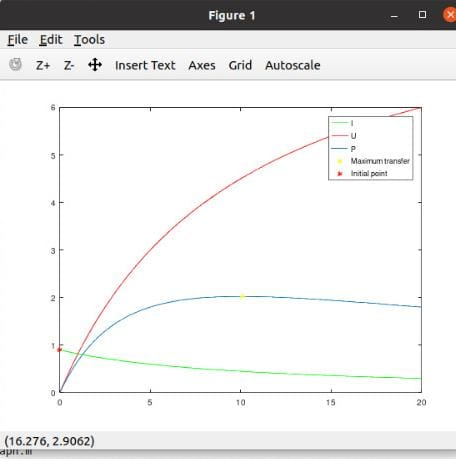
\includegraphics[scale=1]{graph1.jpeg}
\newpage
The OCTAVE function:\\ \\
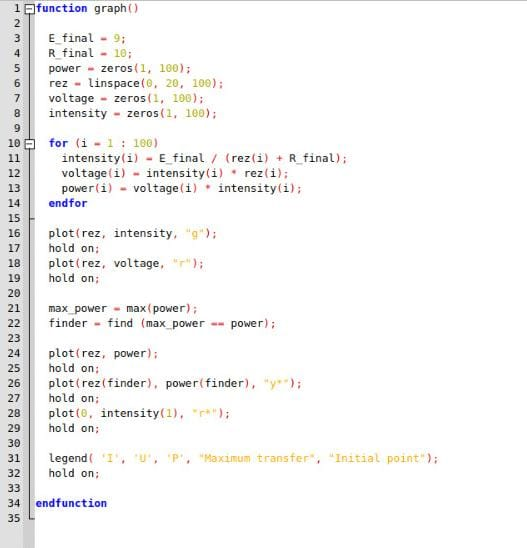
\includegraphics[scale=0.9]{fct1.jpeg}

\newpage
\section{Dependent sources. Spice simulation of dependent sources circuits}
\subsection{SUCU}
The equivalent circuit with a voltage controlled source:\\
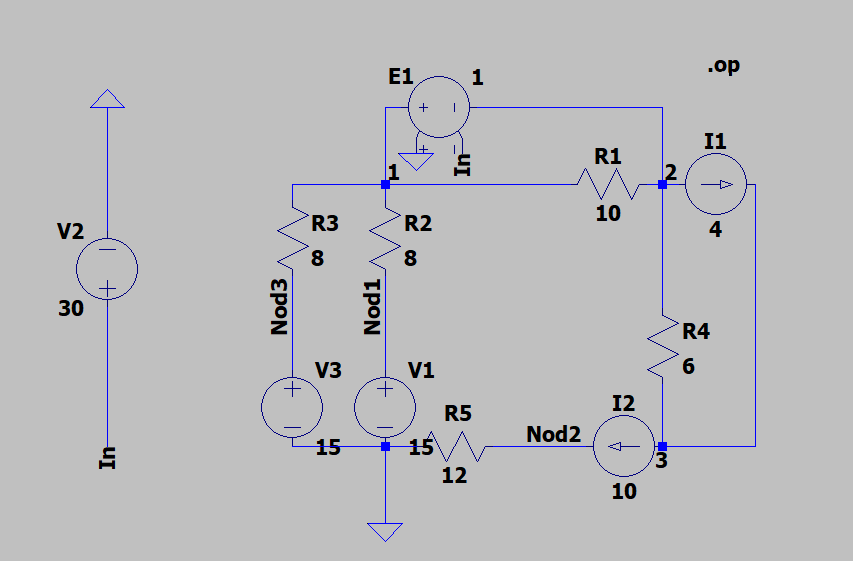
\includegraphics [scale=0.7]{spice.JPG}

\subsection{Diagram}
The diagram, corresponding to the circuit in the figure above is: \\
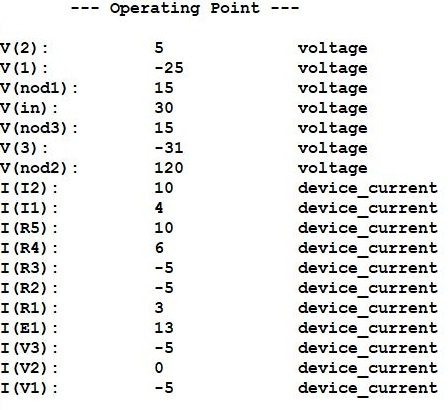
\includegraphics[width=15cm, height=15cm]{net.jpg}\\
\newpage
\section{Solving alternating current circuits using numerical software tools}
The sinusoidal circuit:
\begin{center}
\begin{circuitikz}[european]
\draw (0, 2) to[R, l_=$R_3$,a^=8<\ohm>] (0, 4);
\draw (0,2) to[V<=21.2sin(100$\pi$)V] (0,0);
\draw (0,4) to[short] (4,4);
\draw (0,0) to[short] (4,0)node[label={[font=\footnotesize]below:$(4)$}] {};
\draw (4,6.5) to[short] (4,4)node[label={[yshift=0.2cm, xshift=-7]right:$(1)$}]{};\draw[red] (4, 4) to[R, l_=$R_2$,a^=8<\ohm>, color=red] (4, 2.5);
\draw[red] (4, 2.5) to[V<=21.2sin(100$\pi$+$\frac{\pi}{4}$)V, color=red] (4, 0);
\draw[red] (4, 4) to[R, l_=$R_1$,a^=10<\ohm>, color=red] (7, 4);
\draw (4, 0) to[R, l_=$R_5$,a^=12<\ohm>] (6.5, 0);
\draw (6.5,0) to[short] (7.5,0);
\draw (9, 0) to [I>=14.2sin(100$\pi$) A] (7.5,0) {};
\draw[red] (9, 4) to[R, l_=$R_4$,a^=6<\ohm>, color=red] (9, 0);
\draw[red] (7,4) to [american inductor, a^=$\frac{1}{\pi}$H ,color=red](9,4);
\draw (11,4) to[short] (9,4)node[label={[yshift=0.2cm, xshift=-7]right:$(2)$}]{};;
\draw (9,4) to[short] (9,6.5);
\draw (9,6.5) to[V<=42.2sin(100$\pi$)V] (4,6.5);
\draw (11, 0) to[short] (9,0)node[label={[yshift=0.2cm, xshift=-7]right:$(3)$}] {};
\draw (11, 4) to[I>=5.7sin(100$\pi$+$\frac{\pi}{4}$)A] (11, 2) node[label={[font=\footnotesize]}]{};
\draw (11,0) to [C, a^=$\frac{6}{10^{4}\pi}$F] ++(0,2);
\end{circuitikz}
\end{center}
\newpage
The algebraic form of the circuit:
\begin{center}
\begin{circuitikz}[european]
\draw (0, 2) to[R, l_=$R_3$,a^=8<\ohm>] (0, 4);
\draw (0,2) to[V<=$\frac{15\sqrt{2}}{2}$(1+j)V] (0,0);
\draw (0,4) to[short] (4,4);
\draw (0,0) to[short] (4,0)node[label={[font=\footnotesize]below:$(4)$}] {};
\draw (4,6.5) to[short] (4,4)node[label={[yshift=0.2cm, xshift=-7]right:$(1)$}]{};\draw[red] (4, 4) to[R, l_=$R_2$,a^=8<\ohm>, color=red] (4, 2.5);
\draw[red] (4, 2.5) to[V<=$\frac{15\sqrt{2}}{2}$(1+j)V, color=red] (4, 0);
\draw[red] (4, 4) to[R, l_=$R_1$,a^=10<\ohm>, color=red] (7, 4);
\draw (4, 0) to[R, l_=$R_5$,a^=12<\ohm>] (6.5, 0);
\draw (6.5,0) to[short] (7.5,0);
\draw (9, 0) to [I>=10 A] (7.5,0) {};
\draw[red] (9, 4) to[R, l_=$R_4$,a^=6<\ohm>, color=red] (9, 0);
\draw[red] (7,4) to [american inductor, a^=$10j$ ,color=red](9,4);
\draw (11,4) to[short] (9,4)node[label={[yshift=0.2cm, xshift=-7]right:$(2)$}]{};;
\draw (9,4) to[short] (9,6.5);
\draw (9,6.5) to[V<=30V] (4,6.5);
\draw (11, 0) to[short] (9,0)node[label={[yshift=0.2cm, xshift=-7]right:$(3)$}] {};
\draw (11, 4) to[I>=$\frac{4\sqrt{2}}{2}$(1+j)A] (11, 2) node[label={[font=\footnotesize]}]{};
\draw (11,0) to [C, a^=$\frac{-100}{6}$j] ++(0,2);
\end{circuitikz}
\end{center}

For the 2 chosen sections, the Kirchhoff's current law (1st law) is used, and more 
precisely in the \{3\} and \{4\} nodes.
\begin{equation}
\systeme*{
& => {1}:2*\frac{U_{41}+\frac{15\sqrt{2}}{2}(1+j)}{8}=10,           & => {2}:\frac{U{32}}{6}+10=\frac{4\sqrt{2}}{2}(1+j)}
\end{equation}
The results:\\$U_{41}=29,4-10,6j V$ \\and \\ $U_{32}=-43,03+17jV$\\ as can be seen in the voltage graph, written at the beginning.\\ \\
The script for finding out $U_{41}$ +$U_{32}$ :\\
$U_{41}=\frac{40-15*\sqrt{2}*(1+j)}{2} $
\\
$U_{32}=(\frac{4*\sqrt(2)*(1+j)}{2}-10)*6$
\end{document}


